\documentclass[conference]{IEEEtran}
\IEEEoverridecommandlockouts

% Paquetes necesarios
\usepackage[utf8]{inputenc}
\usepackage[spanish]{babel}
\usepackage{amsmath,amssymb,amsfonts}
\usepackage{algorithmic}
\usepackage{graphicx}
\usepackage{textcomp}
\usepackage{xcolor}
\usepackage{url}
\graphicspath{{img/}}
\begin{document}

\title{Agente Inteligente para el Juego Quarto:\\
Análisis Ontológico y Diseño de Búsqueda Adversarial}

\author{\IEEEauthorblockN{Autor Principal}
\IEEEauthorblockA{\textit{Departamento de Inteligencia Artificial} \\
\textit{Universidad Ejemplo}\\
Lima, Perú \\
email@universidad.edu}
}

\maketitle

\begin{abstract}
Este documento presenta el desarrollo de un agente inteligente capaz de jugar al Quarto mediante técnicas de búsqueda adversarial. Se proporciona una representación ontológica completa del dominio del juego, incluyendo conceptos, relaciones y restricciones. El agente implementa algoritmos minimax con poda Alfa-Beta para la toma de decisiones estratégicas, junto con funciones heurísticas específicas para evaluar posiciones del tablero. La arquitectura propuesta integra percepción del estado del juego, razonamiento basado en búsqueda en el espacio de estados, y ejecución de acciones físicas.
\end{abstract}

\begin{IEEEkeywords}
Inteligencia artificial, juegos adversariales, minimax, ontología, Quarto
\end{IEEEkeywords}

\section{Introducción}

El objetivo es desarrollar un agente inteligente capaz de jugar al Quarto contra un oponente humano, interpretando correctamente el estado del juego y tomando decisiones mediante búsqueda en el espacio de estados \cite{muller2009}. Para ello, el agente puede implementar algoritmos clásicos de juegos adversariales (por ejemplo, minimax con poda Alfa-Beta) que analicen las posibles jugadas futuras \cite{santana2012}.

En esencia, el agente debe \textbf{evaluar} el tablero y seleccionar la acción (colocar o elegir pieza) que maximice su probabilidad de victoria. Trabajos previos han demostrado que, con técnicas de búsqueda eficientes y optimizaciones (por ejemplo, poda Alfa-Beta y tablas de transposición), es posible crear un programa capaz de derrotar a jugadores humanos en tiempo real \cite{russell2016}.

Para construir este agente, el analista de conocimiento primero debe:
\begin{enumerate}
\item \textbf{Identificar el problema de la realidad} que desea resolver.
\item \textbf{Generar una abstracción} de esta realidad.
\item \textbf{Representarlo} simbólicamente en un modelo computable.
\end{enumerate}

\section{Descripción del Juego Quarto}

El Quarto se juega en un \textbf{tablero físico de 4×4 casillas} con 16 piezas de madera distintas. Cada pieza tiene cuatro atributos binarios:
\begin{itemize}
\item \textbf{Color}: blanco o negro
\item \textbf{Tamaño}: alto o bajo
\item \textbf{Forma}: cuadrada o redonda
\item \textbf{Solidez}: hueca o sólida
\end{itemize}


\begin{figure}[h!]
	\centering
	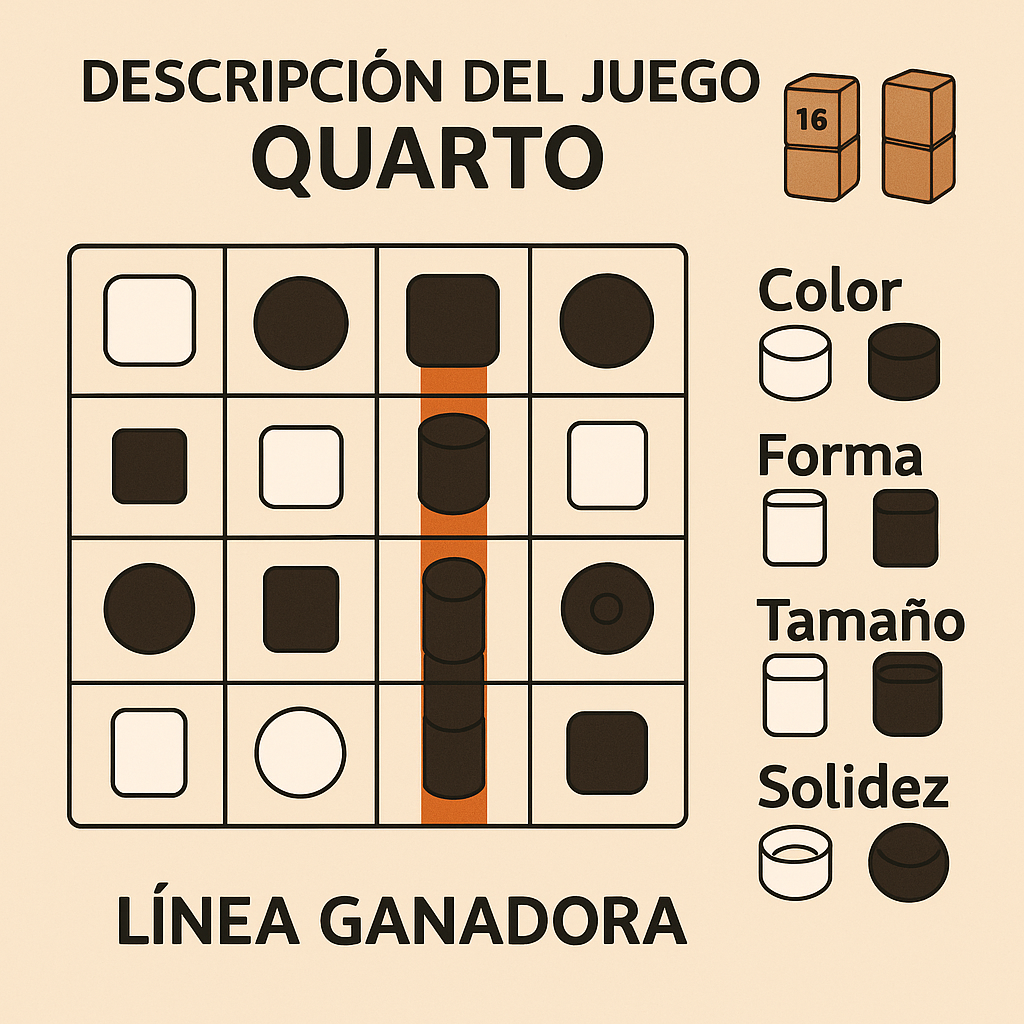
\includegraphics[width=0.48\textwidth]{quarto_tablero.png}
	\caption{Resumen visual del juego Quarto: tablero 4x4, piezas con atributos binarios, y condición de victoria.}
	\label{fig:quarto}
\end{figure}


Así, por ejemplo, puede haber una pieza \textit{blanca, alta, cuadrada y hueca} y otra \textit{negra, baja, redonda y sólida}; todas las 16 combinaciones posibles aparecen exactamente una vez \cite{muller2009}. Al inicio, la bolsa contiene las 16 piezas, y el tablero está vacío.

Los jugadores alternan turnos con una dinámica de "corte y elige": en cada movimiento un jugador \textbf{elige} una pieza disponible y el oponente la \textbf{coloca} en cualquier casilla vacía \cite{santana2012}. Es decir, un turno consta de dos fases: primero se coloca la pieza que quedó "activa" del turno anterior, y luego se selecciona la siguiente pieza que el rival deberá colocar.

Gana el jugador que, al colocar una pieza, completa una línea (horizontal, vertical o diagonal) de cuatro piezas que compartan al menos un atributo. Si el tablero se llena sin que nadie logre esto, la partida termina en empate \cite{muller2009}.



La complejidad combinatoria del Quarto es muy elevada: se estima en torno a $(16!)^2 \approx 4.4 \times 10^{26}$ partidas posibles si se considerara el espacio completo sin podas \cite{santana2012}. Esta cifra incluye todas las secuencias de elección y colocación de piezas (sin contar simetrías), lo que hace inabarcable una búsqueda exhaustiva del espacio completo.



\section{Representación De La Realidad}

La representación de la realidad para el agente se basa en un \textbf{modelo simbólico} que capture el estado del juego.



\begin{figure}[h!]
	\centering
	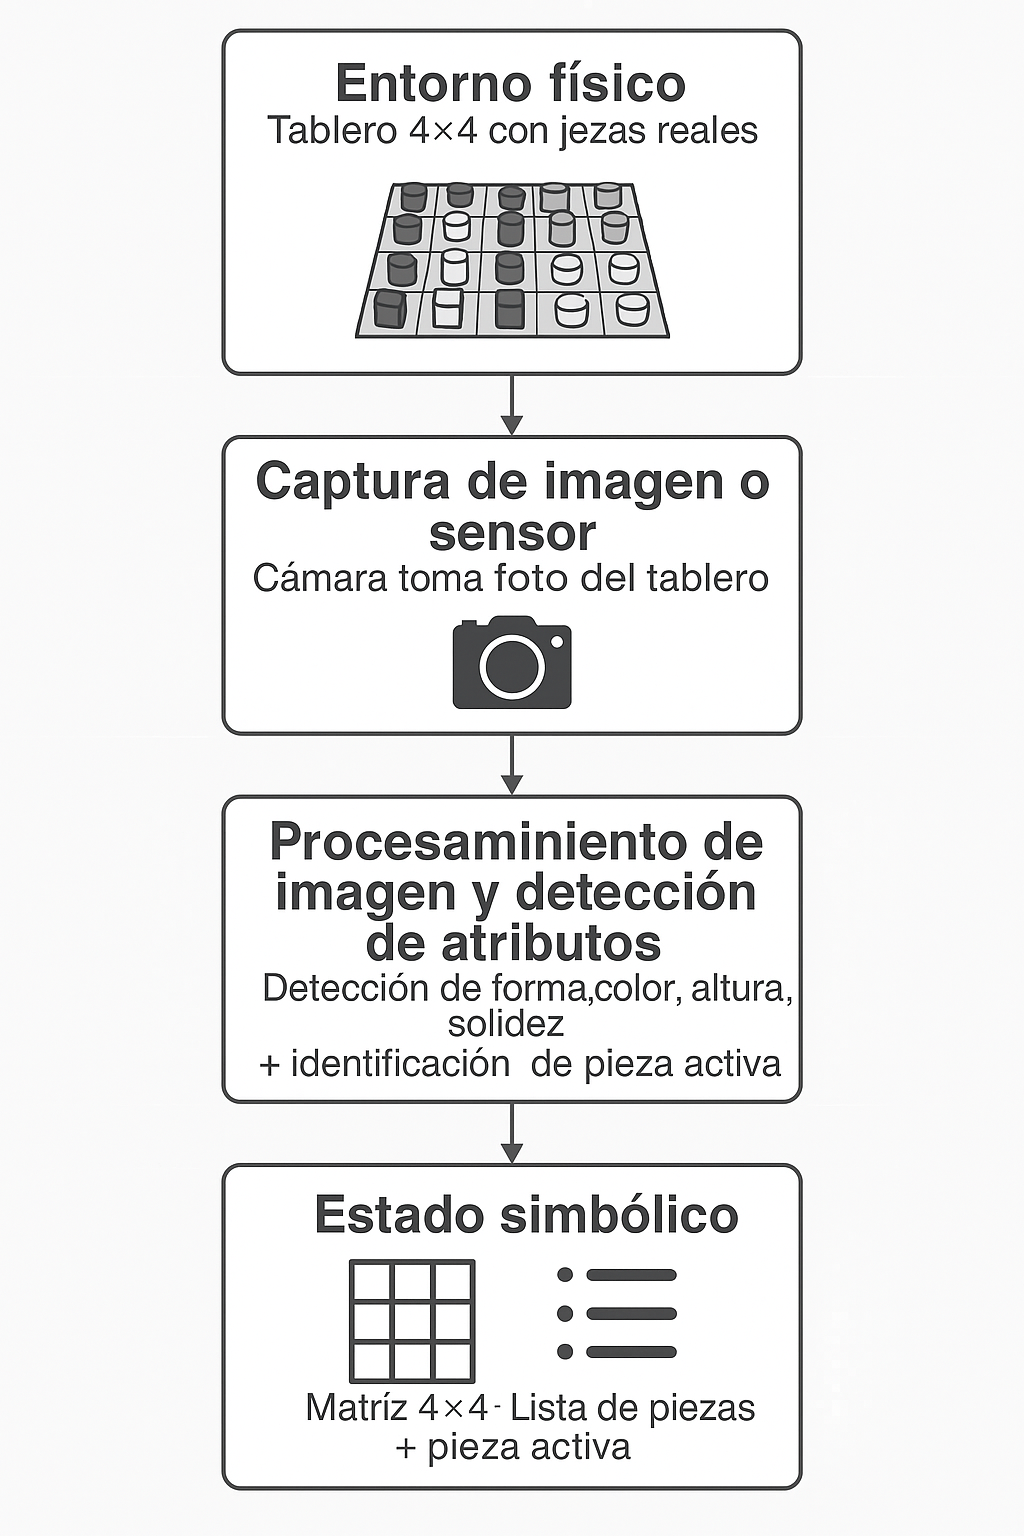
\includegraphics[width=0.95\linewidth]{img/representacion-realidad.png}
	\caption{Representación de la realidad para el agente inteligente en el juego Quarto. Se observa la secuencia: entorno físico, percepción mediante sensor, procesamiento de imagen, construcción del estado simbólico y ejecución de la acción física.}
	\label{fig:representacion_realidad}
\end{figure}

	\subsection{Modelo de Tablero}
	El tablero se representa como una matriz 4×4 de casillas. Cada casilla puede estar vacía o contener una pieza identificada por un código único (1–16).

\subsection{Codificación de Piezas}
Cada pieza se codifica como un vector de 4 bits (uno por cada atributo: color, tamaño, forma, solidez), o bien como un identificador de objeto que contenga esas propiedades. Los 16 identificadores (p. ej., P1, P2, …, P16) corresponden a las 16 combinaciones binarias posibles \cite{muller2009}.

\subsection{Estado de Juego}
El estado del juego incluye:
\begin{itemize}
\item Conjunto de 16 casillas con asignación (vacía o con pieza X)
\item Lista de piezas \textbf{disponibles} (las que aún no se han colocado)
\item Pieza "activa" que debe jugarse en el turno actual
\end{itemize}

\subsection{Percepción y Procesamiento}
El agente utiliza un sensor (por ejemplo, una cámara) para leer la disposición real de piezas en el tablero y su identificación. Mediante técnicas de visión por computador, el agente clasifica color y forma, y deduce el identificador de cada pieza física.





\section{Definición Ontológica}

La definición ontológica describe los elementos esenciales del dominio \textbf{Quarto}, sus relaciones y restricciones.

\subsection{Conceptos Principales}

\begin{itemize}
\item \textbf{Pieza}: Objeto con los atributos $\{\text{color}, \text{tamaño}, \text{forma}, \text{solidez}\}$. Cada combinación binaria es única.
\item \textbf{Casilla}: Posición del tablero identificada por coordenadas $(fila, columna)$ con valores del 1 al 4.
\item \textbf{Tablero}: Conjunto de 16 casillas organizadas en forma matricial 4×4.
\item \textbf{Jugador}: Actor que realiza alternadamente dos acciones: \textit{colocar} una pieza y \textit{elegir} la próxima pieza para el rival.
\item \textbf{Movimiento}: Asociación $\{pieza, casilla\}$ que resulta en colocar una pieza en una casilla vacía.
\item \textbf{Turno}: Ciclo de dos subacciones: colocar la pieza activa en el tablero y elegir la siguiente pieza para el oponente.
\end{itemize}

\subsection{Relaciones}

\begin{itemize}
\item \textbf{ocupa(pieza, casilla)}: Indica que cierta pieza está actualmente en esa casilla.
\item \textbf{disponible(pieza)}: Indica que la pieza aún no ha sido colocada en ninguna casilla.
\item \textbf{vacia(casilla)}: Indica que la casilla no está ocupada.
\item \textbf{pieza-activa(pieza)}: Identifica la pieza que debe colocarse en el turno actual.
\end{itemize}


\begin{figure}[h!]
	\centering
	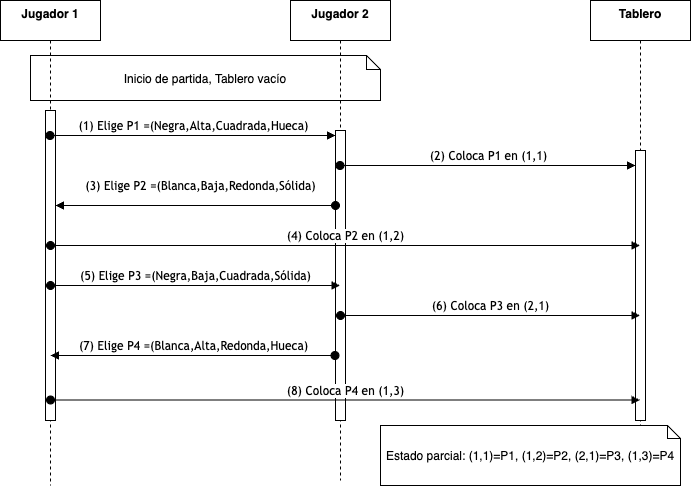
\includegraphics[width=0.95\linewidth]{img/diagrama-secuencia.png}
	\caption{Diagrama de secuencia para las primeras jugadas del juego Quarto entre Jugador 1 y Jugador 2. Se observa la interacción de elección y colocación de piezas en el tablero, con estado parcial al finalizar.}
	\label{fig:secuencia_quarto}
\end{figure}

\subsection{Atributos o Propiedades}
\begin{enumerate}
	
\item \textbf{De las Piezas:}
	\begin{itemize}
		\item \textbf{Color:} Claro / Oscuro
		\item \textbf{Color:} Oscuro
		\item \textbf{Altura:} Alto / Bajo
		\item \textbf{Forma:} Redonda / Cuadrada
		\item \textbf{Solidez:} Hueca / Sólida
	\end{itemize}

	\item \textbf{Del Tablero:}
	\begin{itemize}
		\item \textbf{Tamaño:}  4x4 (16 casillas)
		\item \textbf{Delimitado:} Sí, espacio fijo
	\end{itemize}

	\item \textbf{Del Turno:}
	\begin{itemize}
		\item \textbf{Número de turno}
		\item \textbf{Jugador activo}
		\item \textbf{Pieza colocada}
		\item \textbf{Casilla ocupada}
	\end{itemize}
\end{enumerate}


\subsection{Restricciones del Dominio}

\begin{itemize}
\item Cada \textbf{Pieza} solo puede ser ``disponible'' u ``ocupa'' una única casilla, nunca dos.
\item Una \textbf{Casilla} solo puede contener a lo sumo una pieza.
\item No puede haber dos piezas idénticas en el juego (las 16 combinaciones son disjuntas).
\item Al finalizar un turno, \texttt{pieza-activa} cambia a otra pieza que el jugador elige para el rival.
\item \textbf{Condición de victoria}: existe al menos una línea de cuatro casillas contiguas (horizontal, vertical o diagonal) que contengan piezas con un atributo binario idéntico \cite{muller2009}.
\end{itemize}

\subsection{Consideraciones adicionales}
\begin{itemize}

		\item El \textbf{espacio} de trabajo está previamente delimitado (tablero 4x4).
		\item El juego es de información completa: ambos \textbf{jugadores} ven todas las \textbf{piezas} y el \textbf{tablero}.
		\item \textbf{No hay elementos aleatorios} ni ocultos.
		\item La estrategia se basa en \textbf{anticipación, análisis de patrones y control del turno}.

\end{itemize}


\section{Diseño del Agente de Búsqueda}

El agente inteligente se estructura en tres bloques principales: \textbf{Percepción}, \textbf{Razonamiento (Búsqueda Adversarial)} y \textbf{Acción}.


\begin{figure}[h!]
	\centering
	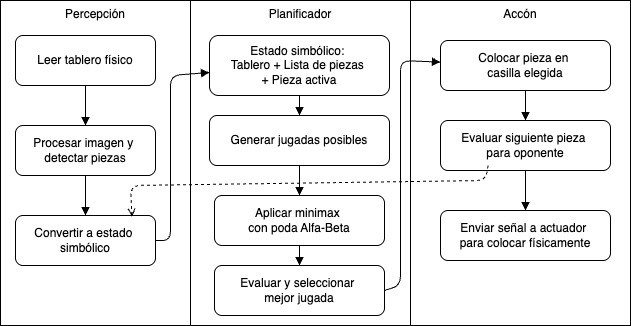
\includegraphics[width=0.95\linewidth]{img/diagrama-busqueda.png}
	\caption{Diagrama de flujo del agente inteligente para el juego Quarto, estructurado en tres fases: Percepción, Planificación y Acción. Se detalla el ciclo de lectura del entorno físico, razonamiento con poda Alfa-Beta y ejecución de acciones físicas.}
	\label{fig:diagrama_busqueda}
\end{figure}

\subsection{Tipo de Agente}
\begin{itemize}
	\item \textbf{Proactivo:} El agente anticipa posibles jugadas del oponente y planifica en consecuencia.
	\item \textbf{Basado en utilidad:} Evalúa el estado del tablero y selecciona acciones que maximizan su probabilidad de victoria.
\end{itemize}

\subsection{Medio Ambiente}
\begin{itemize}
	\item \textbf{Accesible:} El agente tiene acceso completo a toda la información del tablero y las piezas son visibles.
	\item \textbf{Determinista:} Las acciones tienen resultados predecibles.
	\item \textbf{No Episódico:} Las decisiones actuales dependen de estados anteriores.
	\item \textbf{Estático:} El entorno no cambia mientras el agente decide.
	\item \textbf{Discreto:} El número de piezas, casillas y turnos es finito y contable.
\end{itemize}

\subsection{Sensores}

El agente puede utilizar una cámara para capturar una imagen del estado actual del tablero, y luego procesar esta imagen utilizando técnicas de visión por computadora para obtener la siguiente información:

\begin{itemize}
	\item \textbf{Posición de las piezas:} Identificación de las casillas ocupadas por las piezas, a partir de la imagen capturada.
	\item \textbf{Características de las piezas:} Reconocimiento de color, forma, altura y textura.
	\item \textbf{Estado de las casillas:} Detección de casillas vacías o ocupadas.
	\item \textbf{Análisis de patrones:} Identificación de posibles alineaciones de piezas y predicción de jugadas futuras.
\end{itemize}

\subsection{Percepciones}

\begin{itemize}
	\item \textbf{Frecuencia de muestreo:} Cada turno.
	\item \textbf{Número de canales:} 3 (tablero, pieza recibida, piezas disponibles).
	\item \textbf{Dimensiones:} 4x4 para el tablero, 1 para la pieza recibida, hasta 16 para piezas disponibles.
	\item \textbf{Excepciones:} Error si se recibe una pieza ya jugada o si se intenta colocar en una casilla ocupada.
\end{itemize}

\subsection{Percepción del Estado}

\begin{enumerate}
\item \textbf{Leer tablero físico}: Capturar imagen o leer sensor que detecta las 16 casillas.
\item \textbf{Procesar imagen y detectar piezas}: Clasificar cada casilla como ``vacía'' u ``ocupada'' y, si está ocupada, identificar atributos para asignar el código de pieza correcto \cite{muller2009}.
\item \textbf{Convertir a estado simbólico}: Actualizar la matriz 4×4 y la lista de piezas no jugadas.
\end{enumerate}

\subsection{Espacio de Estados}

Número de estados posibles:

	\begin{itemize}
		\item 16 piezas $\rightarrow$ 16! formas de jugarlas.
		\item 16 posiciones en el tablero $\rightarrow$ 16! formas de colocarlas.
		\item Total, aproximado: $(16!)^2 \approx 2.6 \times 10^{36}$ estados posibles.
	\end{itemize}

Esto refleja la complejidad combinatoria del juego.

\subsection{Generación de Jugadas Posibles}

Dado el estado simbólico y la \textit{pieza activa}, el agente obtiene todas las casillas vacías. Cada casilla vacía $c$ genera una jugada candidata $(pieza\_activa, c)$.

\subsection{Algoritmo Minimax con Poda Alfa-Beta}

\subsubsection{Función de Evaluación Heurística}
\begin{itemize}
\item Si un movimiento conduce a una condición definitiva de victoria para el agente, asignar valor $+\infty$.
\item Si permite al oponente ganar inmediatamente, asignar valor $-\infty$.
\item Para estados no terminales, usar una heurística basada en el número de líneas de 3 piezas con posibilidad de completarse.
\end{itemize}

La heurística se define como:
\begin{equation}
h(s) = W_{\text{agente}}(s) - W_{\text{oponente}}(s)
\end{equation}

donde $W$ suma puntajes parciales de líneas de 3 piezas con atributos compartidos \cite{santana2012}.

\subsubsection{Expansión del Árbol de Juego}
\begin{itemize}
\item El estado inicial se expande generando nodos hijos para cada jugada $(pieza\_activa, casilla)$.
\item Para cada hijo, se determina la nueva pieza activa que el adversario recibirá.
\item El árbol crece alternando capas "colocación" y "elección de pieza".
\item Se podan ramas cuyo valor máximo/mínimo no influirá en la decisión final \cite{russell2016}.
\end{itemize}

\subsection{Selección de Pieza para el Oponente}



Después de colocar la pieza en la mejor casilla, el agente debe seleccionar la siguiente pieza que dará al rival:


\begin{enumerate}
\item \textbf{Evaluar cada pieza restante}: Para cada pieza $p$ en la lista de disponibles, simular que el oponente la coloca en las mejores casillas posibles para él.
\item \textbf{Escoger pieza "segura"}: Entre las piezas que no permiten victoria inmediata al rival, seleccionar la que minimice las oportunidades futuras del oponente \cite{santana2012}.
\item \textbf{Asignar pieza activa}: La pieza seleccionada se marca como la nueva pieza activa para el oponente.
\end{enumerate}


\begin{figure}[h!]
	\centering
	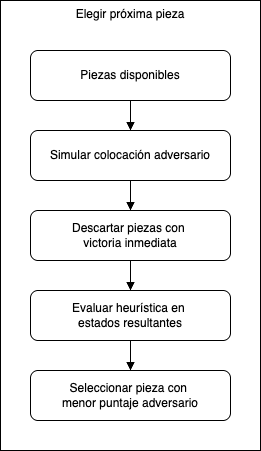
\includegraphics[width=0.95\linewidth]{img/asignar-pieza.png}
	\caption{Subproceso para seleccionar la próxima pieza.}
	\label{fig:asignar_pieza}
\end{figure}

\subsection{Ejecución Física de la Acción}

Una vez decidida la jugada $(pieza\_activa, casilla\_sel)$, se envía la orden al actuador (brazo robótico o interfaz gráfica) para colocar la pieza en la casilla. A continuación, se actualiza la lista de piezas disponibles y la pieza activa pasa a ser el identificador $p_{sel}$ que se dio al oponente.


\section{Medida de Racionalidad}

Para evaluar la racionalidad del agente (su capacidad de tomar decisiones autónomas cercanas a un comportamiento ideal), proponemos los siguientes estadísticos:

\subsection{Tasa de victoria}

\textbf{Descripción:} Porcentaje de partidas ganadas frente a oponentes de referencia. \\
\textbf{Fórmula:}
\begin{equation}
	\text{Tasa de victoria} = \frac{\text{Victorias}}{\text{Total de partidas}} \times 100\%
\end{equation}
\textbf{Justificación:} Mide la eficacia competitiva del agente. \\
\textbf{Fuente:} \cite{herik2002games}

\subsection{Razón de optimalidad de movimiento}

\textbf{Descripción:} Porcentaje de movimientos que coinciden con la acción óptima de un minimax exhaustivo. \\
\textbf{Fórmula:}
\begin{equation}
	\text{Razón de optimalidad} = \frac{\text{Movimientos óptimos}}{\text{Movimientos evaluados}} \times 100\%
\end{equation}
\textbf{Justificación:} Evalúa cuán frecuentemente el agente toma decisiones óptimas. \\
\textbf{Fuente:} \cite{schaeffer1997chinook}

\subsection{Regret promedio}

\textbf{Descripción:} Diferencia entre el valor de la acción óptima y la acción elegida. \\
\textbf{Fórmula:}
\begin{equation}
	\text{Regret promedio} = \frac{1}{N} \sum_{i=1}^{N} \left(V^*(s_i) - V_A(s_i)\right)
\end{equation}
\textbf{Justificación:} Cuanto menor, mayor racionalidad. \\
\textbf{Fuente:} \cite{savage1954foundations}

\subsection{Profundidad de búsqueda promedio}

\textbf{Descripción:} Promedio de niveles explorados en el árbol de búsqueda. \\
\textbf{Fórmula:}
\begin{equation}
	\text{Profundidad promedio} = \frac{1}{N} \sum_{i=1}^{N} d_i
\end{equation}
\textbf{Fuente:} \cite{russell2016artificial}

\subsection{Nodos expandidos promedio por turno}

\textbf{Descripción:} Media de nodos evaluados por turno. \\
\textbf{Fórmula:}
\begin{equation}
	\text{Nodos promedio} = \frac{1}{N} \sum_{i=1}^{N} n_i
\end{equation}
\textbf{Fuente:} \cite{russell2016artificial}

\subsection{Tiempo de decisión promedio}

\textbf{Descripción:} Tiempo promedio en tomar una decisión. \\
\textbf{Fórmula:}
\begin{equation}
	\text{Tiempo promedio} = \frac{1}{N} \sum_{i=1}^{N} t_i
\end{equation}
\textbf{Fuente:} \cite{campbell2002deep}

\subsection{Tasa de empates}

\textbf{Descripción:} Proporción de partidas empatadas. \\
\textbf{Fórmula:}
\begin{equation}
	\text{Tasa de empates} = \frac{\text{Empates}}{\text{Total de partidas}} \times 100\%
\end{equation}
\textbf{Fuente:} \cite{silver2016mastering}

\subsection*{Resumen de métricas}

\begin{table}[h]
	\centering
	\caption{Métricas de racionalidad propuestas}
	\begin{tabular}{|l|c|c|}
		\hline
		\textbf{Métrica} & \textbf{Fórmula} & \textbf{Fuente} \\
		\hline
		Tasa de victoria & $\frac{\#\text{Victorias}}{\#\text{Partidas}} \times 100\%$ & \cite{herik2002games} \\
		Optimalidad de movimiento & $\frac{\#\text{Óptimos}}{\#\text{Evaluados}} \times 100\%$ & \cite{schaeffer1997chinook} \\
		Regret promedio & $\frac{1}{N} \sum(V^* - V_A)$ & \cite{savage1954foundations} \\
		Profundidad promedio & $\frac{1}{N} \sum d_i$ & \cite{russell2016artificial} \\
		Nodos promedio & $\frac{1}{N} \sum n_i$ & \cite{russell2016artificial} \\
		Tiempo promedio & $\frac{1}{N} \sum t_i$ & \cite{campbell2002deep} \\
		Tasa de empates & $\frac{\#\text{Empates}}{\#\text{Partidas}} \times 100\%$ & \cite{silver2016mastering} \\
		\hline
	\end{tabular}
\end{table}



\section{Plan de Implementación del Agente para el Juego Quarto}

\subsection{Descripción General}

Este documento describe el plan de implementación de un agente jugador de \textbf{Quarto} utilizando técnicas de búsqueda adversarial. El agente cuenta con dos modalidades de interacción: una interfaz gráfica basada en \textit{Tkinter} y una interfaz de línea de comandos para propósitos de depuración y análisis.

\subsection{Componentes Principales}

\subsubsection{Estructura de Clases}

\begin{figure}[htbp]
	\centering
	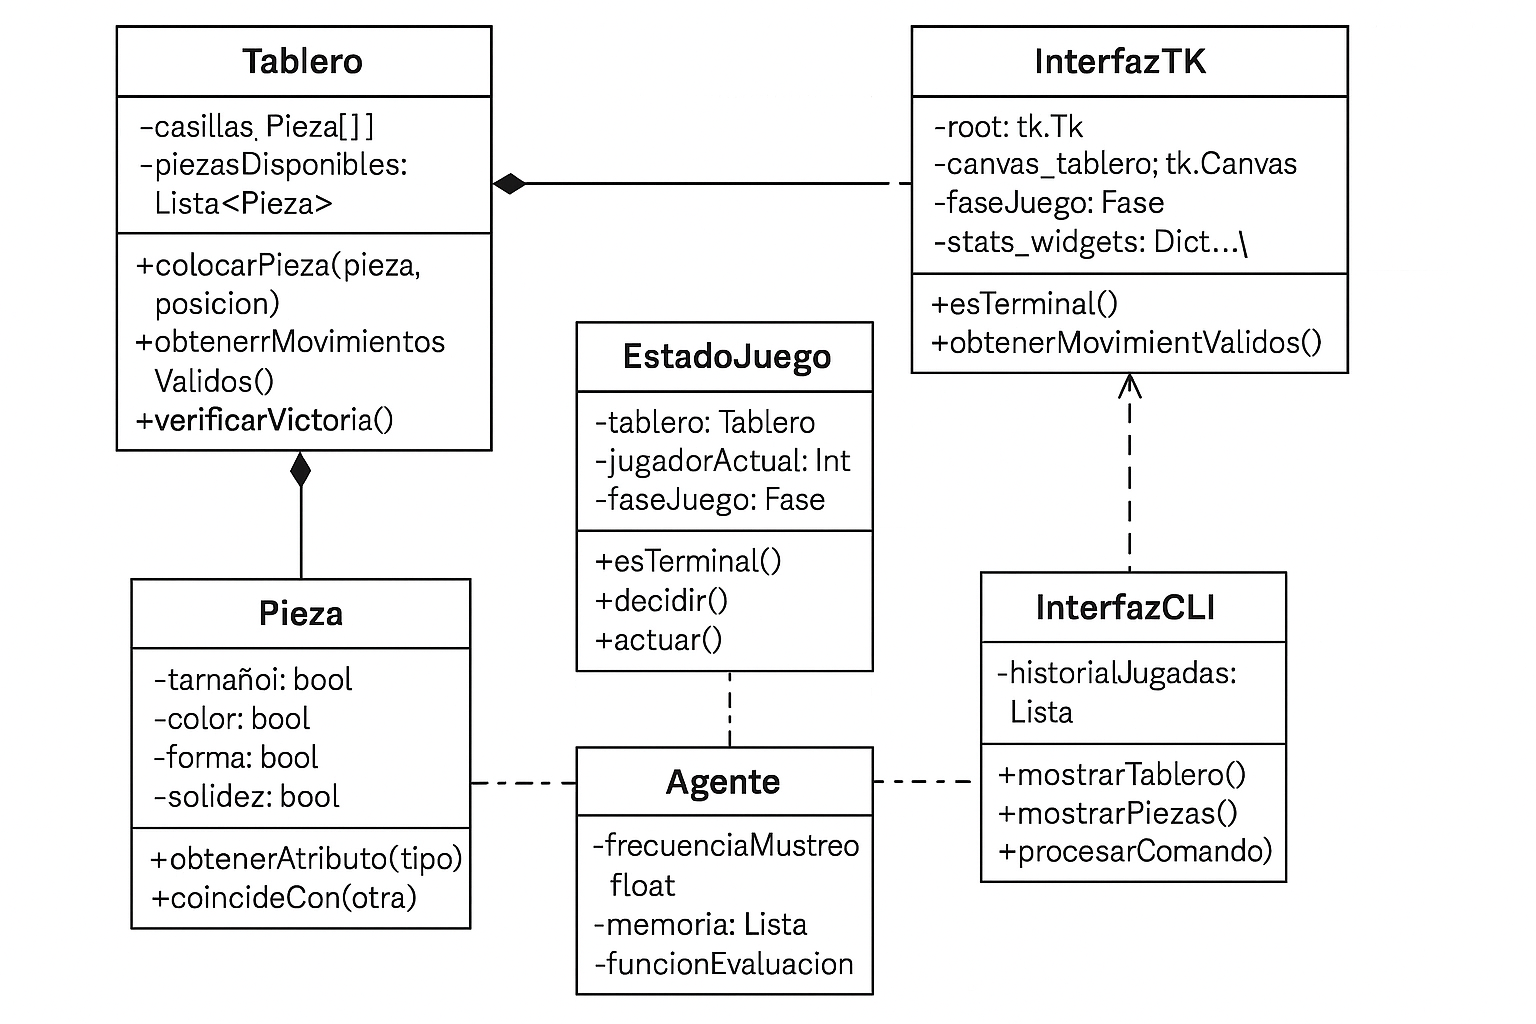
\includegraphics[width=\linewidth]{diagrama-clases.png}
	\caption{Diagrama de clases del agente para el juego Quarto}
	\label{fig:diagrama-clases}
\end{figure}

\section{Diseño del Agente}

\subsection{Tipo de Agente}
\begin{itemize}
	\item \textbf{Clasificación Principal}: Agente Proactivo
	\item \textbf{Clasificación Secundaria}: Agente basado en Objetivos
	\begin{itemize}
		\item Utiliza minimax con poda alfa-beta
		\item Mantiene representación interna del estado
		\item Evalúa estados futuros para lograr victoria
	\end{itemize}
\end{itemize}

\subsection{Características del Entorno}
\begin{enumerate}
	\item \textbf{Accesibilidad}: Accesible. Estado completo del tablero visible, atributos de todas las piezas conocidos, fase actual del juego clara.
	\item \textbf{Determinismo}: Determinista. Acciones con resultados predecibles.
	\item \textbf{Estructura de Episodios}: Secuencial. Historia del juego impacta decisiones.
	\item \textbf{Dinamismo}: Estático. Solo cambia por acciones del agente oponente.
	\item \textbf{Espacio de Estados}: Discreto. Posiciones y combinaciones finitas.
\end{enumerate}

\section{Interfaces de Usuario}

\subsection{Interfaz Gráfica (Tkinter)}
\begin{itemize}
	\item \textbf{Componentes Visuales}: Paneles para tablero, piezas, estado y estadísticas.
	\item \textbf{Interacción}: Mouse para seleccionar y colocar piezas, botones para reiniciar o salir.
	\item \textbf{Código Representativo}:
	\begin{verbatim}
		class InterfazTK:
		def __init__(self):
		self.root = None
		self.canvas_tablero = None
		self.canvas_piezas = None
		self.stats_widgets = {}
		self.historial_jugadas = []
		
		def _dibujar_tablero(self):
		# Renderiza el tablero 4x4 y piezas
		pass
		
		def _dibujar_piezas(self):
		# Muestra piezas disponibles
		pass
		
		def _update_info(self):
		# Actualiza estado e indicadores
		pass
	\end{verbatim}
\end{itemize}

\subsection{Interfaz CLI}
\begin{itemize}
	\item \textbf{Visualización}: ASCII del tablero, lista de piezas y estado del juego.
	\item \textbf{Comandos}: \texttt{colocar X Y}, \texttt{seleccionar N}, \texttt{mostrar}, \texttt{salir}.
\end{itemize}

\section{Sensores y Percepciones}

\subsection{Sensores}
\begin{itemize}
	\item \textbf{Sensor de Tablero}: Lee posiciones y actualiza matriz 4x4.
	\item \textbf{Seguidor de Piezas}: Rastrea atributos y estado de disponibilidad.
\end{itemize}

\subsection{Percepciones}
\begin{itemize}
	\item \textbf{Estructura}: Matriz 4x4, lista de piezas disponibles, pieza activa, fase del juego.
	\item \textbf{Muestreo}: Frecuencia 1/T Hz, canales: tablero, piezas, fase.
\end{itemize}

\section{Monitoreo y Estadísticas}

\subsection{Estadísticas en Tiempo Real}
Decisiones tomadas, tiempo promedio, nodos explorados, podas realizadas.

\subsection{Capturas y Logs}
Capturas automáticas, logs de jugadas y estadísticas finales.

\section{Estructura de Archivos}
\begin{verbatim}
	quarto/
	    src/
	        juego/
				__init__.py
				tablero.py
				pieza.py
				estado.py
			agente/
				__init__.py
				agente.py
			interfaces/
				__init__.py
				tk_gui.py
				cli.py
			utils/
				__init__.py
				constantes.py
		tests/
			test_juego.py
			test_agente.py
			test_interfaces.py
		README.md
		requirements.txt
\end{verbatim}

\section{Dependencias}
\subsection{Bibliotecas}
Tkinter, PIL, Time, Logging

\subsection{Herramientas}
Python 3.8+, pytest, Black, pylint

\section{Secuencia de Implementación}

\subsection{Fase 1: Lógica Base}
\begin{itemize}
	\item Implementación del Tablero
	\item Clase Pieza con atributos
	\item Gestión básica de estado
	\item Verificación de victoria
\end{itemize}

\subsection{Fase 2: Interfaces}
\begin{itemize}
	\item Implementación CLI
	\item GUI con Tkinter
	\item Sistema de estadísticas
	\item Capturas y logs
\end{itemize}

\subsection{Fase 3: Agente}
\begin{itemize}
	\item Sistema de percepción
	\item Validación de acciones
	\item Representación de estado
	\item Toma de decisiones
\end{itemize}

\subsection{Fase 4: Optimización}
\begin{itemize}
	\item Eficiencia de memoria
	\item Poda de búsqueda
	\item Ajuste de heurísticas
	\item Métricas de rendimiento
\end{itemize}


\section{Manual del Proyecto: Juego Quarto con Agente Inteligente}

\subsection{Resumen}
Implementación del juego Quarto con un agente inteligente basado en búsqueda adversarial usando minimax con poda alfa-beta.

\subsection{Características Principales}
\begin{itemize}
	\item Interfaz gráfica con Tkinter
	\item Interfaz de línea de comandos
	\item Agente inteligente proactivo basado en objetivos
	\item Búsqueda adversarial con minimax y poda alfa-beta
	\item Frecuencia de muestreo configurable
	\item Estadísticas de rendimiento del agente integradas
	\item Capturas automáticas del juego
\end{itemize}

\subsection{Requisitos}
\begin{itemize}
	\item Python 3.8 o superior
	\item Paquetes requeridos:
	\begin{itemize}
		\item \texttt{pillow} (para capturas)
		\item \texttt{pytest} (para pruebas)
		\item \texttt{black} (para formateo)
		\item \texttt{pylint} (para análisis de código)
	\end{itemize}
\end{itemize}

\subsection{Instalación}
\begin{enumerate}
	\item Clonar el repositorio:
	\begin{verbatim}
		git clone <url-repositorio>
		cd quarto
	\end{verbatim}
	
	\item (Opcional) Crear un entorno virtual:
	\begin{verbatim}
		python -m venv venv
		source venv/bin/activate  # Linux/Mac
		venv\Scripts\activate     # Windows
	\end{verbatim}
	
	\item Instalar dependencias:
	\begin{verbatim}
		pip install -r requirements.txt
	\end{verbatim}
\end{enumerate}

\subsection{Modo de Uso}

\paragraph{Ejecución por defecto:}
\begin{verbatim}
	python main.py
\end{verbatim}

\paragraph{Modo CLI:}
\begin{verbatim}
	python main.py --modo cli
\end{verbatim}

\paragraph{Opciones adicionales:}
\begin{itemize}
	\item \texttt{--modo}: Selecciona el modo de interfaz (tk/cli)
	\item \texttt{--frecuencia}: Frecuencia del agente en Hz (por defecto: 1.0)
	\item \texttt{--primer\_jugador}: Jugador que inicia la partida (humano/agente)
\end{itemize}

\textbf{Ejemplos:}
\begin{verbatim}
	python main.py --modo tk --primer_jugador agente
	python main.py --modo tk --frecuencia 0.5
\end{verbatim}

\subsection{Reglas del Juego}

\subsubsection{Tablero y Piezas}
\begin{itemize}
	\item Tablero de 4x4 casillas
	\item 16 piezas únicas con 4 atributos binarios:
	\begin{itemize}
		\item Tamaño: Grande/Pequeña
		\item Color: Roja/Azul
		\item Forma: Redonda/Cuadrada
		\item Solidez: Sólida/Hueca
	\end{itemize}
\end{itemize}

\subsubsection{Mecánica de Juego}
\begin{enumerate}
	\item Los jugadores alternan turnos
	\item Cada turno tiene dos fases:
	\begin{itemize}
		\item \textbf{Colocar:} Poner la pieza activa en el tablero
		\item \textbf{Seleccionar:} Elegir la próxima pieza para el rival
	\end{itemize}
\end{enumerate}

\subsubsection{Condición de Victoria}
Completar una línea de 4 piezas (horizontal, vertical o diagonal) con al menos un atributo común. Si el tablero se llena sin victoria, se declara empate.

\subsection{Interfaz Gráfica}

\paragraph{Disposición:}
\begin{itemize}
	\item Panel izquierdo: Tablero 4x4
	\item Panel central: Piezas disponibles y log
	\item Panel derecho: Estado del juego y estadísticas
\end{itemize}

\paragraph{Controles:}
\begin{itemize}
	\item Click izquierdo para seleccionar o colocar piezas
	\item Botón Reiniciar: Nueva partida
	\item Botón Salir: Cierra la aplicación
\end{itemize}

\paragraph{Funciones destacadas:}
\begin{itemize}
	\item Resaltado visual de selección
	\item Indicadores de fase y turno
	\item Estadísticas en tiempo real
	\item Capturas automáticas (opcional)
	\item Guardado de logs y estadísticas
\end{itemize}

\subsection{Interfaz de Línea de Comandos}

\paragraph{Comandos disponibles:}
\begin{itemize}
	\item \texttt{mostrar}: Ver estado actual
	\item \texttt{seleccionar N}: Seleccionar pieza número N
	\item \texttt{colocar F C}: Colocar pieza en fila F, columna C
	\item \texttt{ayuda}: Mostrar instrucciones
	\item \texttt{salir}: Terminar el juego
\end{itemize}

\subsection{Agente Inteligente}

\paragraph{Características:}
\begin{itemize}
	\item Agente proactivo basado en objetivos
	\item Estrategia: minimax con poda alfa-beta
	\item Percepción del entorno mediante muestreo configurable
\end{itemize}

\paragraph{Heurísticas:}
\begin{itemize}
	\item Evaluación de líneas con atributos compartidos
	\item Bloqueo de posibles victorias del oponente
	\item Maximización de oportunidades propias
\end{itemize}

\subsection{Estructura del Proyecto}
\begin{verbatim}
	quarto/
		src/
			juego/
				pieza.py
				tablero.py
				estado.py
			agente/
				agente.py
			interfaces/
				tk_gui.py
				cli.py
		tests/
		main.py
		requirements.txt
		README.md
\end{verbatim}

\subsection{Contribución}
\begin{enumerate}
	\item Crear un fork del repositorio
	\item Crear una rama para tu nueva característica
	\item Realizar commits con los cambios
	\item Crear un pull request para revisión
\end{enumerate}



\section{Conclusiones}

Se ha presentado un marco completo para el desarrollo de un agente inteligente para el juego Quarto, incluyendo una representación ontológica detallada del dominio y un diseño de arquitectura basado en búsqueda adversarial. La implementación del algoritmo minimax con poda Alfa-Beta, junto con funciones heurísticas específicas, permite al agente tomar decisiones estratégicas eficientes en tiempo real.

La complejidad combinatoria del Quarto requiere el uso de técnicas de poda y limitación de profundidad para hacer viable la búsqueda en el espacio de estados. El enfoque propuesto integra exitosamente la percepción del estado físico del juego con el razonamiento simbólico y la ejecución de acciones.

\begin{thebibliography}{9}
	
	\bibitem{muller2009}
	B. Müller, \textit{Quarto – Análisis del juego y estrategias de búsqueda}. Barcelona: Ediciones Gigamic, 2009.
	
	\bibitem{russell2016}
	S. J. Russell and P. Norvig, \textit{Artificial Intelligence: A Modern Approach}, 3rd ed. Pearson, 2016.
	
	\bibitem{savage1954}
	L. J. Savage, \textit{The Foundations of Statistics}. New York: Wiley, 1954.
	
	\bibitem{campbell2002}
	M. Campbell, A. J. Hoane, and F. H. Hsu, \textit{Deep Blue}. Artificial Intelligence, vol. 134, no. 1–2, pp. 57–83, 2002.
	
	\bibitem{schaeffer1997}
	J. Schaeffer, R. Lake, P. Lu, and M. Bryant, \textit{Chinook: The world man–machine checkers champion}. AI Magazine, vol. 18, no. 1, pp. 21–29, 1997.
	
	\bibitem{silver2016}
	D. Silver et al., \textit{Mastering the game of Go with deep neural networks and tree search}. Nature, vol. 529, no. 7587, pp. 484–489, 2016.
	
	\bibitem{herik2002}
	H. J. van den Herik, J. W. H. M. Uiterwijk, and J. van Rijswijck, \textit{Games solved: A success story}. International Computer Games Association Journal, vol. 25, no. 3, pp. 178–189, 2002.
	
	\bibitem{santana2012}
	J. Santana and M. López, \textit{Algoritmos adversariales para juegos de mesa: Aplicación en Quarto}. Revista Iberoamericana de Inteligencia Artificial, vol. 14, no. 2, pp. 45–58, 2012.
	
\end{thebibliography}








\end{document}